
\begin{figure}[t]
\centering
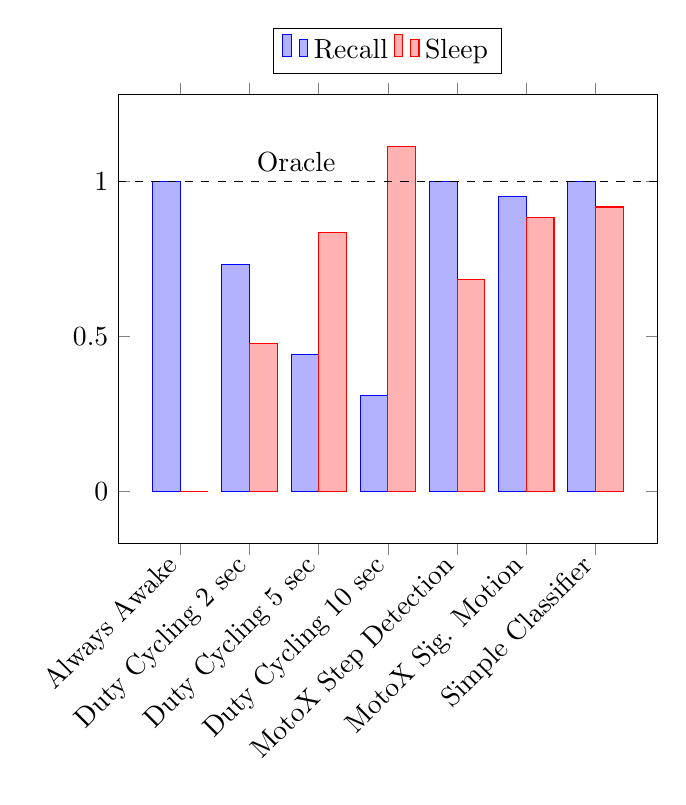
\begin{tikzpicture}
\begin{axis}[
	ybar=0pt,% space of 0pt between adjacent bars
	enlargelimits=0.15,
	legend style={at={(0.5,1.15)},anchor=north,legend columns=-1},
	symbolic x coords={
		Always Awake,
		Duty Cycling 2 sec,
		Duty Cycling 5 sec,
		Duty Cycling 10 sec,
		MotoX Step Detection,
		MotoX Sig. Motion,
		Simple Classifier},
	x tick label style={rotate=45,anchor=east},
	xtick=data,
	%nodes near coords,
	nodes near coords align={vertical},
]
\addplot coordinates {
	(Always Awake,1.0) 
	(Duty Cycling 2 sec,0.73) 
	(Duty Cycling 5 sec,0.44) 
	(Duty Cycling 10 sec,0.31)
	(MotoX Step Detection, 1.0)
	(MotoX Sig. Motion, 0.95)
	(Simple Classifier, 1.0)};
\addplot coordinates {
	(Always Awake,0.0) 
	(Duty Cycling 2 sec,0.476667) 
	(Duty Cycling 5 sec,0.833333) 
	(Duty Cycling 10 sec,1.111111) 
	(MotoX Step Detection, 0.683)
	(MotoX Sig. Motion, 0.883333)
	(Simple Classifier, 0.916667)};
\draw [black, dashed] ({rel axis cs:0,0}|-{axis cs:Always Awake,1}) -- ({rel axis cs:1,0}|-{axis cs:Always Awake,1}) node [pos=0.33, above] {Oracle};
\legend{Recall,Sleep}
\end{axis}
\end{tikzpicture}
\caption{Footstep Detection}
\label{table:footstepDetectionRecallSleepTime}
\end{figure}


\begin{figure}[t]
\centering
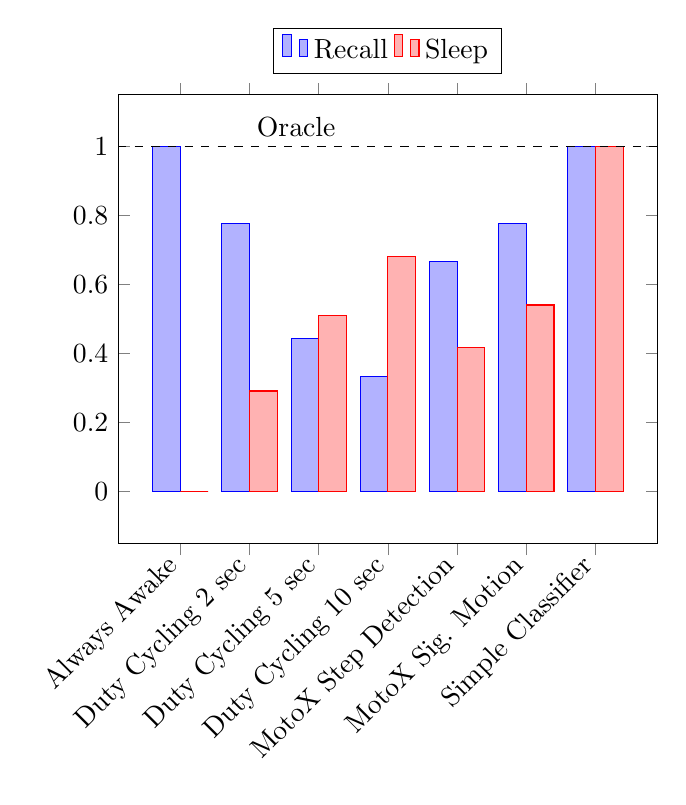
\begin{tikzpicture}
\begin{axis}[
	ybar=0pt,% space of 0pt between adjacent bars
	enlargelimits=0.15,
	legend style={at={(0.5,1.15)},anchor=north,legend columns=-1},
	symbolic x coords={
		Always Awake,
		Duty Cycling 2 sec,
		Duty Cycling 5 sec,
		Duty Cycling 10 sec,
		MotoX Step Detection,
		MotoX Sig. Motion,
		Simple Classifier},
	x tick label style={rotate=45,anchor=east},
	xtick=data,
	%nodes near coords,
	nodes near coords align={vertical},
]
\addplot coordinates {
	(Always Awake,1) 
	(Duty Cycling 2 sec,0.7778) 
	(Duty Cycling 5 sec,0.4444) 
	(Duty Cycling 10 sec,0.3333) 
	(MotoX Step Detection,0.6667)
	(MotoX Sig. Motion, 0.7778)
	(Simple Classifier, 1)};
\addplot coordinates {
	(Always Awake,0.0) 
	(Duty Cycling 2 sec,0.291545) 
	(Duty Cycling 5 sec,0.510204) 
	(Duty Cycling 10 sec,0.680272) 
	(MotoX Step Detection, 0.418367)
	(MotoX Sig. Motion, 0.540816)
	(Simple Classifier, 1)};
\draw [black, dashed] ({rel axis cs:0,0}|-{axis cs:Always Awake,1}) -- ({rel axis cs:1,0}|-{axis cs:Always Awake,1}) node [pos=0.33, above] {Oracle};
\legend{Recall,Sleep}
\end{axis}
\end{tikzpicture}
\caption{Fall Detection {\em TODO please drop Always Awake from the graph and add results for batching.  Add some pattern to the bars so that they are readable even when printing in balck and white.  }}
\label{table:fallDetectionRecallSleepTime}
\end{figure}


\section{Evaluation}
\label{sec:validation}

Defining the set of algorithms that should be implemented by the
platform and defining the API is beyond the scope of this position
paper.  Instead, this section provides evidence to support our
conjecture.  We use trace-based simulation to evaluate the performance
of two simple classifiers built using common pre-processing algorithms
for two accelerometer-based applications.


\subsection{Applications}

We developed two applications that detect activities performed by 
human subjects:

\begin{enumerate}
\setlength{\itemsep}{-3pt}  

\item A {\em Step Detector} based on the human step detection algorithm
  proposed by Ryan Libby in~\cite{libbyFootstepDetection}. {\em TODO you need to say more about how this works.  Don't assume thst the reader is familiar with the reference}.

\item A {\em Fall Detector} based on a simple thresholding algorithm,
  as described in~\cite{kangasFallDetection}.  {\em TODO same as
    previous comment}

\end{enumerate}

\subsection{Configurations}

We evaluate the recall and prevision of step and fall detection under the following configurations:

\begin{itemize}

\item Duty Cycle {\em TODO add 1 sentence examplanation}

\item Batching {\em TODO add 1 sentence examplanation}

\item MotoX Step Detections {\em TODO add examplanation that describes that we use the builtin step detector to wake up the device and then run the main app, be it step detection or fall detection.}

\item MotoX Significant Motion {\em TODO add examplanation that describes that we use the builtin significant motion API to wake up the device and then run the main app, be it step detection or fall detection.}

\item Simple Classifier {\em TODO describe the algorithms that we assume are supported by the platform for each stage (noise-reduction, feature extraction, admission control).  Then briefly describe how we implemented two classifiers for the two apps by configuring this algorithms.} 

\end{itemize}

\subsection{Traces}

We collected two traces from human subjects using a Motorola Moto X
device, running Android 4.4.4.  The smartphone ran an application that
kept the device always awake and continuously recorded all raw
accelerometer readings, as well as {\em step} and {\em significant
  motion} events, which are supported natively by the Moto X.

The first trace is 10 minutes long and consists of readings taken from
a person walking, standing idle, falling to the groud, and performing
other activities (e.g., seating down, standing up, taking the device
out of the pocket). This trace was carefully engineered so that
walking and falling account for 40\% and 2\% of the trace,
respectively.  This was done to allow us to evaluate the performance
of applications that track frequent as well as unfrequent events.  We
collected this trace in a controlled environment which enabled us to
annotate it with high quality ground truth data.

The second trace is 2 hours and 50 minutes long and captures one of
the author's morning routine (getting ready, having breakfast and
commuting to work). This trace was not annotated with ground truth
information, but enable evaluate the applications under more realistic
conditions.

\subsection{Results}

Figures~\ref{table:footstepDetectionRecallSleepTime}
and~\ref{table:fallDetectionRecallSleepTime} show the recall and
achieved sleep time for step and fall detection for the 10 minutes
long traces.  Results are normalized by the recall and sleep time of a
hypothetical ideal implementation that only wakes up when an event of
interest occurs.  The ideal implementation sleeps for 60\% and 98\% of
the time for step detection and fall detection, respectively.

As expected, Duty Cycling is effective at reducing the amount of time
the device is awake (and thus, power consumption), but performs poorly
in terms of event of interest recall.  Similarly, batching achieves
good recall, but has poor sleep performance, specially for infrequent
events, such as fall detection.


{\em TODO discuss how motox step detection works for steps and falls.}

{\em TODO discuss results of motox significant motion works for steps
  and falls.  Also discuss performance for second trace.}


{\em TODO present the results of simple classifier for both traces.
  Also make the point that the performance of this approach is so good
  that there is little additional benefit to be gained from general
  programability.}







 